\documentclass{beamer}
\usepackage{indentfirst}
\usepackage{tabularx}
\usepackage{graphicx}
\usepackage{caption}
\usepackage{amsmath}
\usepackage{siunitx}
\usepackage{babel}
\usepackage{hyperref}
\hypersetup{
	colorlinks=true,
	urlcolor=blue,
  linkcolor=black,
}
%\titleformat{\chapter}{\normalfont\huge\bfseries}{\thechapter.}{1em}{}
%\renewcommand\thechapter{\arabic{chapter}.}
\sisetup{output-decimal-marker={,}}
\newcommand{\ifig}[1]{
  \begin{figure}[h!]
    \fbox{\includegraphics[width=1\textwidth]{#1}}
  \end{figure}
}

\usetheme{JuanLesPins}
\usecolortheme{crane}
\beamertemplatenavigationsymbolsempty

\title[]{Wayland}
\subtitle{A modern display protocol for Linux}
\author{Ioan-Alexandru Popa}
\institute{Faculty of Automatic Control and Computers, CB Series, 322CB Group}
\date{January 18, 2024}

\begin{document}

\frame{\titlepage}

\begin{frame}
  \frametitle{Table of contents}
  \tableofcontents
\end{frame}

\section{X11 -- the original display protocol}
\begin{frame}
  \frametitle{X11 -- the original display protocol}
  \begin{columns}[T]
    \begin{column}{0.7\textwidth}
      \begin{itemize}
        \item Created in 1984 as part of MIT's Project Athena
        \item Optimized for the low-powered PC's available at that time
        \item Designed to display apps running on other computers
        \item Based on a client-server architecture
      \end{itemize}
    \end{column}
    \begin{column}{0.3\textwidth}
      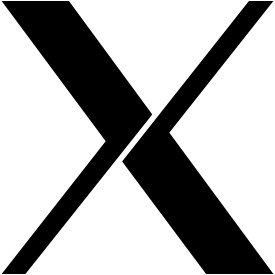
\includegraphics[width=\textwidth]{X11_Logo.png}

      \textit{\footnotesize The X11 logo}
    \end{column}
  \end{columns}
\end{frame}

\begin{frame}
  \frametitle{The X server}
      \begin{itemize}
        \item Grants clients access to GUI resources (screen space, keyboard, etc.)
        \item \textbf{Many} components, like the window manager (which handles the windows' layout and title bars), are mere \textbf{clients}
      \end{itemize}
  \begin{center}
    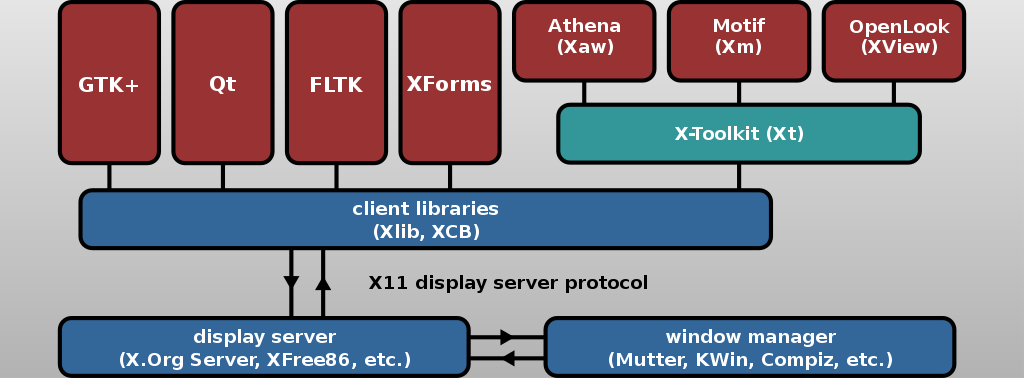
\includegraphics[width=\textwidth]{X11_Diagram.png}
  \end{center}
\end{frame}

\begin{frame}
  \frametitle{The X.Org server}
  \begin{columns}[T]
    \begin{column}{0.7\textwidth}
      \begin{itemize}
        \item The X.Org server is the canonical X server implementation
        \item \textbf{Ugly code} that barely anyone wants to develop besides the Red Hat employees paid to do that
        \item Any X server \textbf{has} to implement a \textbf{plethora of features} and extensions to be compatible, some seldomly used
        \item No one wants to develop new X servers anymore
      \end{itemize}
    \end{column}
    \begin{column}{0.3\textwidth}
      
\includegraphics[width=\textwidth]{X.Org_Logo.png}

      \textit{\footnotesize The X.Org logo}
    \end{column}
  \end{columns}
\end{frame}

\begin{frame}
  \frametitle{Issues of the X11 protocol}
  \begin{columns}[T]
    \begin{column}{0.65\textwidth}
      \begin{itemize}
        \item \textbf{Not} designed with \textbf{security} in mind
        \item Makes some \textbf{outdated} assumptions about the \textbf{rendering process}
        \item Has some \textbf{inherent limitations} that can't be overcome without breaking backward compatibility
        \begin{itemize}
          \item All monitors have to have the same DPI
          \item No new modifier keys can be added -- the new Apple laptops can't be fully supported
        \end{itemize}
      \end{itemize}
    \end{column}
    \begin{column}{0.35\textwidth}
      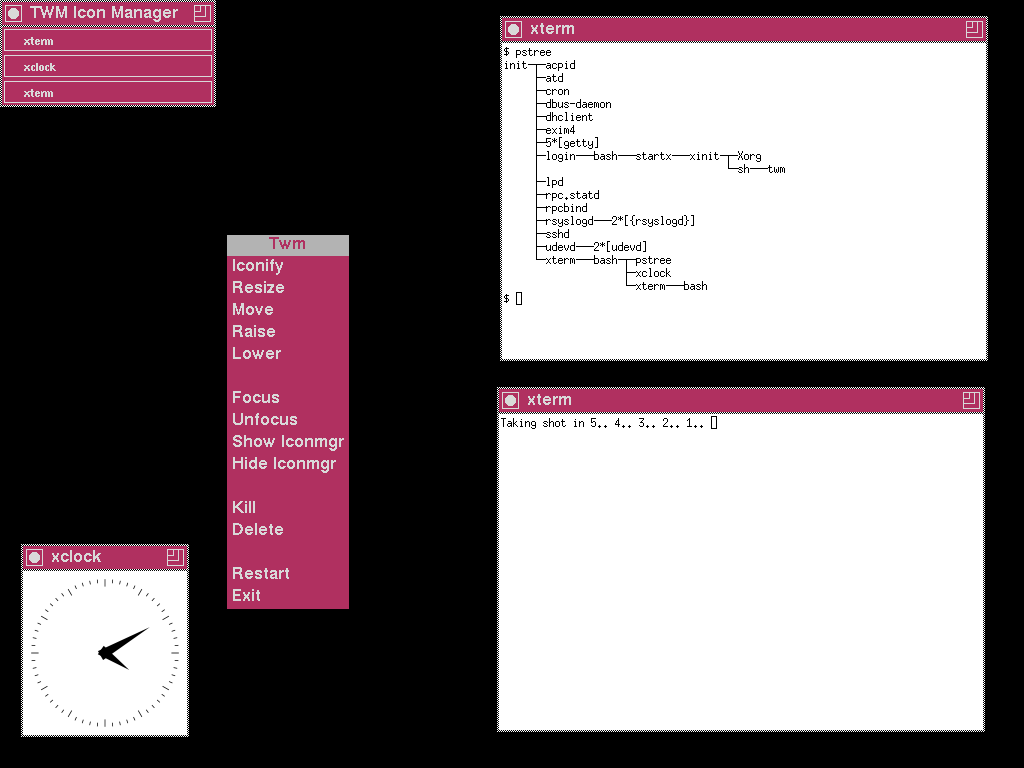
\includegraphics[width=\textwidth]{Debian_TWM_Maroon.png}

      \textit{\footnotesize TWM -- an X11 window manager}
    \end{column}
  \end{columns}
\end{frame}

\section{Wayland -- the better display protocol}
\begin{frame}
  \frametitle{Wayland -- the better display protocol}
  \begin{columns}[T]
    \begin{column}{0.7\textwidth}
      \begin{itemize}
        \item Created in 2008 by Kristian Høgsberg
        \item \textbf{Addresses} many of X11's \textbf{flaws}
        \item \textbf{Tightly couples} the display server, compositor and window manager
        \item Most X.Org developers are now working on Wayland instead
      \end{itemize}
    \end{column}
    \begin{column}{0.3\textwidth}
      
\includegraphics[width=\textwidth]{Wayland_Logo.png}

      \textit{\footnotesize The Wayland logo}
    \end{column}
  \end{columns}
\end{frame}

\begin{frame}
  \frametitle{How Wayland works}
  \centering
  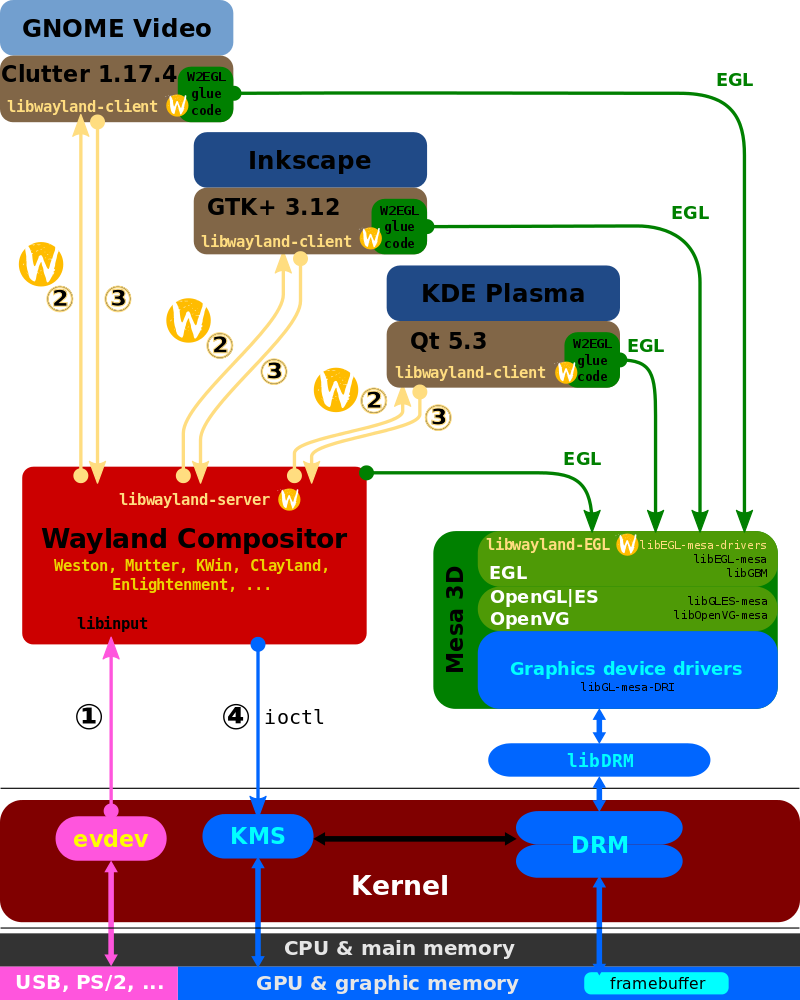
\includegraphics[height=0.85\textheight]{Wayland_Diagram.png}
\end{frame}

\begin{frame}
  \frametitle{Wayland implementations}
  \begin{columns}[T]
    \begin{column}{0.7\textwidth}
  \begin{itemize}
    \item Gnome (Mutter) -- the default environment on Ubuntu
    \item KDE Plasma (KWin) -- another popular desktop environment
    \item Weston -- the reference implementation
    \item Sway -- a minimalist, i3-like environment
    \begin{itemize}
      \item \texttt{wlroots} is a popular library for building Wayland compositors
    \end{itemize}
  \end{itemize}
    \end{column}
    \begin{column}{0.3\textwidth}
      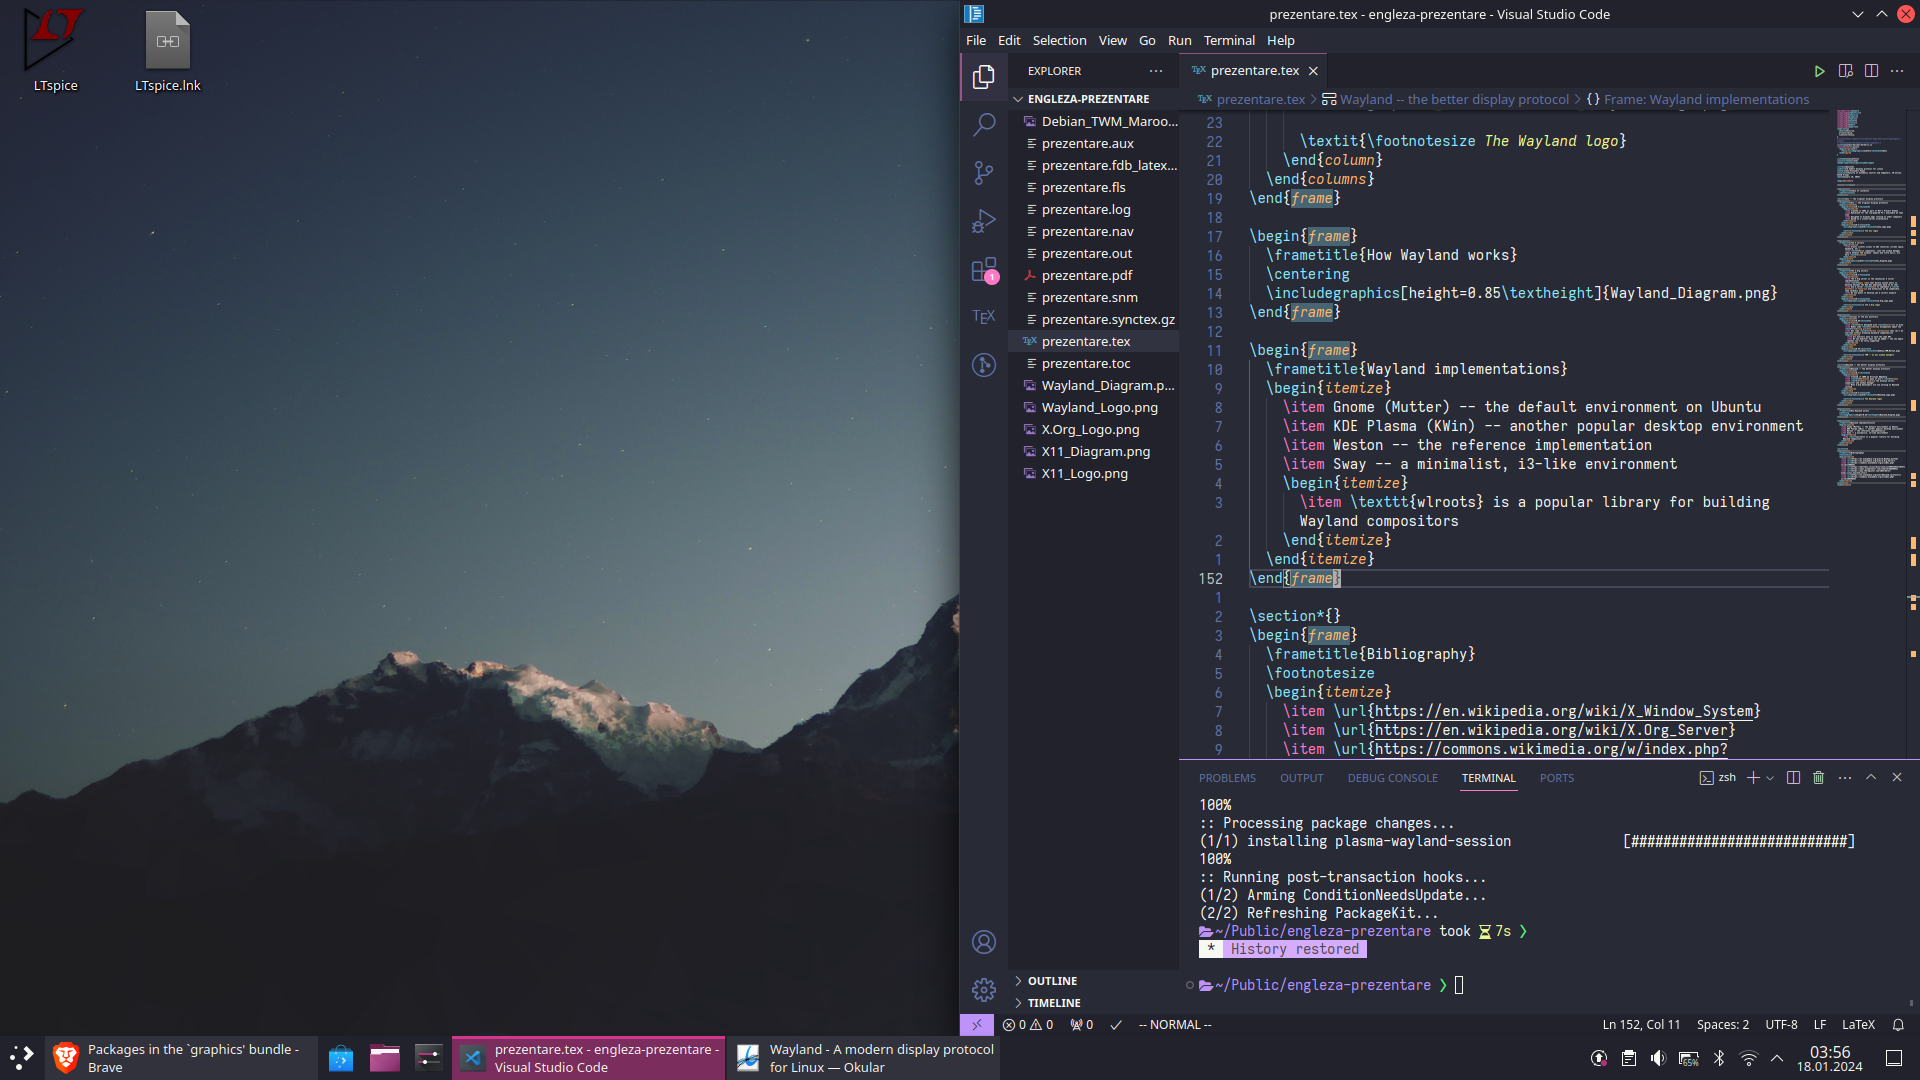
\includegraphics[width=\textwidth]{KDE_Wayland.png}

      \textit{\footnotesize KDE Plasma 5}
    \end{column}
  \end{columns}
\end{frame}

\begin{frame}
  \frametitle{The state of Wayland}
  \begin{itemize}
    \item Many functionalities are implemented using portals
    \begin{itemize}
      \item Global hotkeys, screen capture, etc.
      \item They are designed with \textbf{security in mind}; the user can tweak the \textbf{app permissions}
      \item Some things are still not fully fleshed out, but work is in progress
    \end{itemize}
    \item Gnome, Fedora strongly favor Wayland
    \begin{itemize}
      \item Even Ubuntu now ships with Wayland by default
    \end{itemize}
    \item Proprietary Nvidia drivers are almost fully functional
    \begin{itemize}
      \item Some compositors might require some tweaks
    \end{itemize}
  \end{itemize}
\end{frame}

\section{Summary}
\begin{frame}
  \frametitle{Summary}
  \begin{itemize}
    \item X11 is the \textbf{old}, original Linux display protocol
    \begin{itemize}
      \item It's \textbf{outdated}
      \item It desperately needs replacement
    \end{itemize}
    \item Wayland is the \textbf{fresh}, new Linux display protocol
    \begin{itemize}
      \item Made for the 21st century
      \item It's \textbf{the future}, and even the present
    \end{itemize}
  \end{itemize}
\end{frame}

\section{Conclusion}
\begin{frame}
  \frametitle{Conclusion}
  \begin{itemize}
    \item Wayland is ready to be the flagship display protocol of Linux
    \item Fixing X11's flaws definitely requires more work that making Wayland 100\% functional
  \end{itemize}
\end{frame}

\section*{}
\begin{frame}
  \frametitle{Bibliography}
  \footnotesize
  \begin{itemize}
    \item \url{https://en.wikipedia.org/wiki/X_Window_System}
    \item \url{https://en.wikipedia.org/wiki/X.Org_Server}
    \item \url{https://commons.wikimedia.org/w/index.php?curid=1298844}
    \item \url{https://mastodon.social/@csoriano/111489425631719327}
    \item \url{https://news.ycombinator.com/item?id=38639022}
    \item \url{https://www.theregister.com/2023/05/17/asahi_linux_wayland_only/}
    \item \url{https://en.wikipedia.org/wiki/Wayland_(protocol)}
    \item \url{https://commons.wikimedia.org/w/index.php?curid=28029855}
  \end{itemize}
\end{frame}
\end{document}
